% !TEX root = main.tex

\section{线性判别函数} % 5.1-5.8 (5.10-5.12)
% 5.2 线性判别函数和判定面(单类、多类)
% 广义线性判别函数 5.3
% 5.4 两类线性可分情况
%  梯度下降法、牛顿法、Hessian矩阵
% 感知器算法 5.5
% 5.6 松弛算法
% 5.7 不可分情况
% MSE 5.8
%  MSE与Fisher线性判别
% 5.10 线性规划
% SVM 5.11
%  VC Dimension
%  Kernel Trick
%  Soft Margin
% 5.12 拓展到多类
% Model Selection
%  Cross Validation (k-fold)

\subsection{线性判别函数和判定面}
判别(discriminant)函数是指由$\vx$的各个分量线性组合而成的函数
\[g(\vx)=\vw^\T\vx+w_0\]
这里$\vw$是权向量,$w_0$称为阈权值(threshold)或偏置。

对于二类线性分类器来说,$g(\vx)>0$则判为$\omega_1$,否则判为$\omega_2$。
方程$g(\vx)=0$定义了一个判定面,将归类于$\omega_1$和$\omega_2$的点分开来。
当$g(\vx)$是线性的,这个平面称为超平面。

判别函数是特征空间某点$\vx$到超平面距离的代数度量(注意到垂直平行特性)
\[\vx=\vx_p+r\frac{\vw}{\norm{\vw}}\]
其中$\vx_p$是$\vx$在超平面$H$上的投影向量,$r$是相应的算术距离,为正则$\vx$在$H$正侧,否则在$H$负侧。
由于$g(\vx_p)=0$,有
\[g(\vx)=\vw^\T\vx+w_0=r\norm{\vw}\]
或
\[r=\frac{g(\vx)}{\norm{\vw}}\]
\begin{figure}[H]
\centering
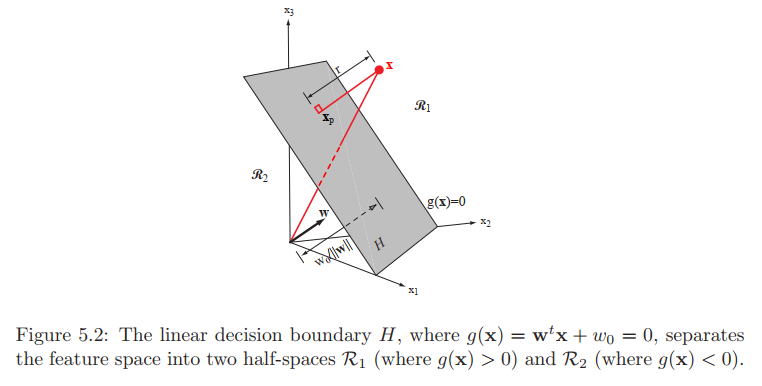
\includegraphics[width=0.9\linewidth]{fig/linear_decision_boundary.png}
\end{figure}

对于多类样本来说,则将$c$类问题转化为$c$个二类问题;或者用$c(c-1)/2$个线性判别函数,将样本分为$c$个类别,每个线性判别函数只对其中两个类别分类。

\subsection{广义线性判别函数}
线性判别函数可写成
\[g(\vx)=w_0+\sum_{i=1}^d w_i x_i\]
系数$w_i$是权向量$\vw$的分量,通过加入另外的项($\vw$的各对分量之间的乘积),得到二次判别函数
\[g(\vx)=w_0+\sum_{i=1}^d w_ix_i+\sum_{i=1}^d\sum_{j=1}^d w_{ij}x_ix_j\]
因$x_ix_j=x_jx_i$,不失一般性假设$w_{ij}=w_{ji}$。

继续加入更高次项(如$w_{ijk}x_ix_jx_k$)可得到多项式判别函数,可看作对某一判别函数$g(x)$做级数展开,然后取截尾逼近,意味着某一广义线性判别函数
\[g(\vx)=\sum_{i=1}^d a_iy_i(\vx)\]
或
\[g(\vx)=\va^\T\vy\]

特别地,线性判别函数可写成
\[g(\vx)=w_0+\sum_{i=1}^d w_i x_i=\sum_{i=0}^dw_ix_i\]
令$\vy=\bmat{1 & \vx}^\T$为\textbf{增广特征向量},$\va=\bmat{w_0 & \vw}$为增广权向量,注意这里是将偏置放在了第$0$位。

对于一个样本$\vy_i$,若$\va^\T\vy_i>0$就标记为$\omega_1$,若$\va^\T\vy_i<0$就标记为$\omega_2$。
这样可以通过一种规范化(normalization)方法来简化两类样本训练过程,即对于属于$\omega_2$的样本,用负号表示而不是标记$\omega_2$(将属于$\omega_2$的样本用$\bmat{-1 & -y_i}^\T$表示)。
这样就可以直接寻找一个对所有样本都有$\va^\T\vy_i>0$的权向量$\va$,这样的向量称为分离(separating)向量或解向量。

求解权向量的过程相当于确定权空间中一点,每个样本都对应解向量的可能位置给出限制。
$\va\vy_i^\T$确定了一个穿过权空间原点的超平面,$\vy_i$为其法向。
解向量若存在,则一定在每个超平面的正侧。
由于是不等式约束,故解不唯一,要加入其他约束条件。
一种方法是找到一个单位长度的权向量,使得从样本到分类平面最小距离达到最大;另一种方法则在所有$i$中寻找满足$\va^\T\vy_i\geq b$的具有最小长度的权向量,这里的$b$是被称为边沿裕量(margin)/间隔的正常数。

求解$\va^\T\vy_i>0$的解所采用的方法是:定义一个准则函数$J(\va)$,当$\va$是解向量时,$J(\va)$最小,因此可将其简化为一个标量函数极小化问题,通常用梯度下降法解决。
\[\va(k+1)=\va(k)-\eta(k)\nabla J(\va(k))\]
其中$\eta$为正的比例因子,即学习率。

假设准则函数可以通过二阶展开近似
\[J(\va)\approx J(\va(k))+\nabla J^\T(\va-\va(k))+\frac{1}{2}(\va-\va(k))^\T H(\va-\va(k))\]
即当选择
\[\eta(k)=\frac{\norm{\nabla J}^2}{\nabla J^T H\nabla J}\]
时,可使$J(\va(k+1))$最小化。

牛顿法
\[\va(k+1)=\va(k)-H^{-1}\nabla J\]

\subsection{感知器}
考虑构造线性不等式$\va^\T\vy_i>0$的准则函数,用错分的样本作为准则函数不好因为分段常数不利于梯度搜索。
更好的选择是感知器(perceptron)准则函数
\[J_p(\va)=\sum_{\vy\in\mY}(-\va^\T\vy)\]
这里$\mY(\va)$是被$\va$错分的样本集。
由几何上知,$J_p(\va)$是与错分样本到判决边界距离之和成正比的。
对上式求导有
\[\nabla J_p=\sum_{\vy\in\mY}(-\vy)\]
得到梯度下降迭代公式
\[\va(k+1)=\va(k)+\eta(k)\sum_{\vy\in\mY_k}\vy\]

\subsection{最小平方误差}
设$Y$为$n\times\hat{d}$的矩阵,$n$为样本数,$\hat{d}=d+1$为维度,第$i$行是向量$\vy_i^\T$,令$\vb=\bmat{b_1 &\cdots & b_n}^\T$,目标是找到权重$\va$满足
\[Y\va=\vb\]
定义误差向量
\[\ve=Y\va-\vb\]
使误差向量长度平方最小化,即最小化平方误差和(MSE)准则函数
\[J_s(\va)=\norm{Y\va-\vb}^2=\sum_{i=1}^n(\va^\T\vy_i-b_i)^2\]
计算梯度有
\[\nabla J_s=2Y^\T(Y\va-\vb)\]
令其为$0$有
\[Y^\T Y\va=Y^\T\vb\]
当方阵$Y^\T Y$非奇异时,有唯一解
\[\va=(Y^\T Y)^{-1} Y^\T\vb=Y^\dag\vb\]
这里的$\hat{d}\times n$矩阵
\[Y^\dag=(Y^\T Y)^{-1} Y^\T\]
称为$Y$的伪逆矩阵。
注意到若$Y$为方阵且非奇异,则这个伪逆矩阵即为$Y$的逆矩阵。
还应注意到$Y^\dag Y=I$,但通常$YY^\dag\ne I$。

MSE与Fisher线性判别函数的解是一样的。

\subsection{支持向量机}
支持向量机(support vector machine, SVM)通过一个足够高维的非线性映射$\varphi(\cdot)$,将两类数据用超平面进行分割。
假设每个模式$\vx_k$变换到$\vy_k=\varphi(\vx_k)$,则问题在于选择$\varphi(\cdot)$。
对$n$个模式中的每一个$k=1,\ldots,n$,根据模式属于$\omega_1$或$\omega_2$,分别令$z_k=\pm 1$,增广空间$\vy$上的判别函数是
\[g(\vy)=\va^\T\vy\]
这里权向量和变换后的模式向量都是增广的(取$a_0=w_0,y_0=1$),则这样的分割超平面保证
\[z_kg(\vy_k)\geq 1,\;k=1,\ldots,n\]
\begin{figure}[H]
\centering
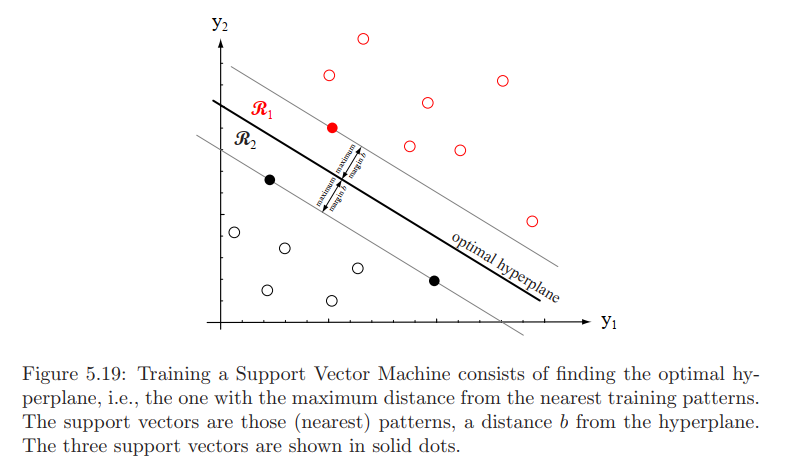
\includegraphics[width=0.9\linewidth]{fig/SVM.png}
\end{figure}

训练一个支持向量机的目标是找到一个具有\textbf{最大间隔}(largest margin)的分割平面,若间隔越大则得到的分类器也越好。
从超平面到变换后的模式$\vy$的距离是$|g(\vy)|/\norm{\va}$(即做投影),若正的间隔$b$存在,则推出
\[\frac{z_kg(\vy_k)}{\norm{\va}}\geq b,\;k=1,\ldots,n\]
目标即找一个使得$b$最大化的权向量$\va$。
由于解向量可以任意伸缩且保持超平面不变,故有限制条件$b\norm{a}=1$,即其确定的是$\norm{\va}$的极小值。

支持向量是使上式等号成立的模式向量,即支持向量是最靠近超平面的,也是最难分类的样本/对求解分类任务最富有信息的模式。

目标为极小化$\norm{\va}$,构造拉格朗日函数
\[L(\va,\valpha)=\frac{1}{2}\norm{\va}^2-\sum_{k=1}^n\alpha_k[z_k\va^\T\vy_k-1]\]
可用KKT条件改写为
\[\begin{aligned}
&L(\valpha)=\sum_{i=1}^n\alpha_i-\frac{1}{2}\sum_{k,j}^n\alpha_k\alpha_jz_kz_j\vy_j^\T\vy_k\\
&s.t.\sum_{k=1}^nz_k\alpha_k=0,\;\alpha_k\geq 0,\;k=1,\ldots,n
\end{aligned}\]
进行求解(先用约束消元,逐一令偏导为$0$求解)。

\subsection{软间隔与正则化}
前面都假定训练样本在样本空间或特征空间中线性可分,然而现实中却很难找到这些线性可分的任务,也很难判定不是由于过拟合造成。
缓解该问题一个方法是允许支持向量机在一些样本上出错,为此引入软间隔(soft margin)概念。
\begin{figure}[H]
\centering
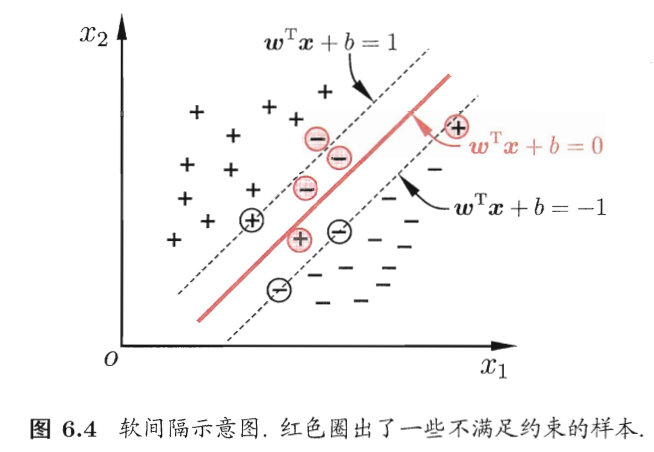
\includegraphics[width=0.6\linewidth]{fig/soft_margin.png}
\end{figure}

允许某些样本不满足不等式约束
\[y_i(\vw^\T\vx_i+b)\geq 1\]
于是在最大化间隔的同时,不满足约束的样本应尽可能少,得到优化目标
\[\min_{\vw,b}\frac{1}{2}\norm{\vw}^2+C\sum_{i=1}^ml_{0/1}(y_i(\vw^\T\vx+b)-1),\,C>0\]
其中$l_{0/1}$为0/1损失函数。

也有其他损失函数
\begin{itemize}
	\item Hinge损失:$l_{hinge}(z)=\max(0,1-z)$
	\item 指数损失:$l_{exp}(z)=\exp(z)$
	\item 对率损失:$l_{log}(z)=\log(1+\exp(-z))$
\end{itemize}

\subsection{核方法}
对变量升维,以便线性划分
\[\kappa(\vx,\vx_i)=\phi(\vx_i)^\T\phi(\vx)\]

\subsection{VC维}
衡量函数复杂性,通过评估函数类中函数的弯曲程度实现。
VC维越大,曲线越弯曲。
\begin{figure}[H]
\centering
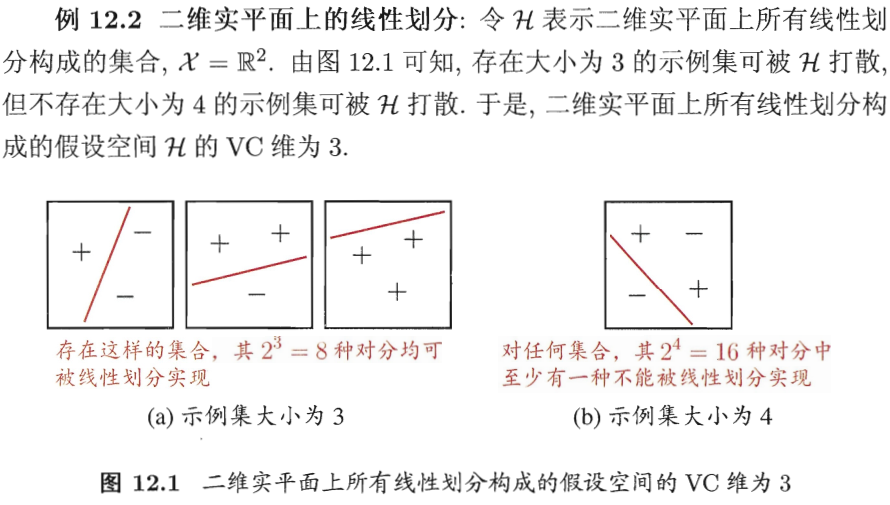
\includegraphics[width=0.6\linewidth]{fig/vc_dimension.png}
\end{figure}